\documentclass[aspectratio=169,14pt]{beamer}
\usetheme{default}\usecolortheme{default}\setbeamertemplate{navigation symbols}{}
\setbeamertemplate{footline}{\hfill{\scriptsize\color{covermuted}\insertframenumber/\inserttotalframenumber}\hspace{0.4cm}\vspace{0.15cm}}
\usepackage{fontspec}\usepackage{xeCJK}\setCJKmainfont{PingFang SC}[BoldFont=PingFang SC Semibold]\setmainfont{Helvetica Neue}[BoldFont=Helvetica Neue Bold]
\usepackage{xcolor}\usepackage{tikz}\usepackage{graphicx}\usepackage{fontawesome5}\usetikzlibrary{positioning,calc,arrows.meta,shadows}
\definecolor{bgmain}{RGB}{238,243,252}\definecolor{panel}{RGB}{238,244,255}\definecolor{factbg}{RGB}{246,242,235}\definecolor{coverprimary}{HTML}{2563EB}\definecolor{coveraccent}{HTML}{00A884}\definecolor{coverwarning}{HTML}{F59E0B}\definecolor{coverdark}{HTML}{1F2937}\definecolor{covermuted}{HTML}{64748B}\definecolor{titlecolor}{RGB}{30,30,30}\definecolor{muteddark}{RGB}{72,86,115}\definecolor{bluepanel}{RGB}{226,237,255}\definecolor{greenpanel}{RGB}{225,246,237}\definecolor{amberpanel}{RGB}{255,244,222}\definecolor{purplepanel}{RGB}{239,231,255}\setbeamercolor{background canvas}{bg=bgmain}
\newcommand{\plainbar}{\begin{tikzpicture}[remember picture, overlay]\fill[coverdark, opacity=0.07] (current page.south west) rectangle ([yshift=0.4cm]current page.south east);\draw[coveraccent, opacity=0.45, line width=0.8pt] ([yshift=0.4cm]current page.south west) -- ([yshift=0.4cm]current page.south east);\end{tikzpicture}}
\newcommand{\deckbackground}{\begin{tikzpicture}[remember picture, overlay]\fill[coverprimary!8] (current page.north west) rectangle (current page.south east);\fill[coverprimary!14] (current page.north west) ++(1.55,-1.35) circle (2.45cm);\fill[coveraccent!12] (current page.south east) ++(-1.9,1.45) circle (2.70cm);\fill[coverwarning!12] (current page.north east) ++(-2.9,-1.8) circle (0.85cm);\foreach \x in {-0.2,0.8,...,16.2} {\draw[coverprimary, opacity=0.045, line width=0.25pt] ([xshift=\x cm]current page.south west) -- ([xshift=\x cm]current page.north west);}\foreach \y in {-0.2,0.7,...,9.3} {\draw[coverprimary, opacity=0.04, line width=0.25pt] ([yshift=\y cm]current page.south west) -- ([yshift=\y cm]current page.south east);}\draw[coveraccent, opacity=0.38, line width=1.1pt] ([xshift=0.35cm,yshift=7.72cm]current page.south west) -- ++(3.25,0) -- ++(0.45,-0.45) -- ++(2.0,0);\draw[coverprimary, opacity=0.24, line width=1.0pt] ([xshift=9.35cm,yshift=8.25cm]current page.south west) -- ++(2.3,0) -- ++(0.55,-0.55) -- ++(3.2,0);\fill[coverdark, opacity=0.07] (current page.south west) rectangle ([yshift=0.42cm]current page.south east);\end{tikzpicture}}
\newcommand{\sectiontitle}[2]{\vspace{-0.52cm}\begin{center}{\fontsize{20}{24}\selectfont\bfseries\color{titlecolor} #1}\\[2pt]{\fontsize{9}{11}\selectfont\itshape\color{muteddark} #2}\end{center}\vspace{0.12cm}}
\newcommand{\portraitbox}[2]{\begin{tikzpicture}\node[draw=coverprimary!28, line width=0.7pt, fill=white, rounded corners=3pt, inner sep=2.5pt, drop shadow={shadow xshift=0.5pt, shadow yshift=-0.5pt, opacity=0.12}] {\includegraphics[width=2.4cm,height=2.9cm,keepaspectratio]{#1}};\end{tikzpicture}{\par\vspace{1pt}\fontsize{6.5}{7.5}\selectfont\color{covermuted} #2\par}}
\newcommand{\placeholderportrait}[2]{\begin{tikzpicture}\node[draw=coverprimary!28, line width=0.7pt, fill=white, rounded corners=3pt, inner sep=2.5pt, drop shadow={shadow xshift=0.5pt, shadow yshift=-0.5pt, opacity=0.12}] {\begin{tikzpicture}\fill[bluepanel] (0,0) rectangle (2.4,2.9);\foreach \x/\y in {0.25/0.45,0.55/1.85,0.95/1.15,1.35/2.2,1.75/0.85,2.1/1.65} {\fill[coverprimary!32] (\x,\y) circle (0.055cm);}\draw[coveraccent!45, line width=0.55pt] (0.25,0.45) -- (0.55,1.85) -- (0.95,1.15) -- (1.35,2.2) -- (1.75,0.85) -- (2.1,1.65);\node[circle, fill=coverprimary!16, minimum size=0.78cm] at (1.2,1.78) {};\node[rounded corners=8pt, fill=coverprimary!16, minimum width=1.28cm, minimum height=0.72cm] at (1.2,0.78) {};\node[font=\fontsize{12}{14}\selectfont\bfseries, text=coverprimary!75!black] at (1.2,0.17) {#1};\end{tikzpicture}};\end{tikzpicture}{\par\vspace{1pt}\fontsize{6.5}{7.5}\selectfont\color{covermuted} #2\par}}
\newcommand{\personslide}[9]{\begin{frame}\plainbar\vspace{-0.45cm}\begin{center}{\fontsize{22}{26}\selectfont\bfseries\color{coverdark} #1}\\[2pt]{\fontsize{9.5}{11.5}\selectfont\color{muteddark} #2}\end{center}\vspace{0.15cm}\begin{columns}[c]\begin{column}{0.22\textwidth}\centering #3\end{column}\begin{column}{0.28\textwidth}\begin{tikzpicture}\node[fill=greenpanel, rounded corners=4pt, inner xsep=6pt, inner ysep=5pt, text width=3.8cm, align=left] {{\fontsize{7}{8.5}\selectfont\bfseries\color{coveraccent!70!black} 获奖}\enspace{\fontsize{7}{8.5}\selectfont\color{coverdark!85} #4}\\[2.5pt]{\fontsize{7}{8.5}\selectfont\bfseries\color{coveraccent!70!black} 生卒}\enspace{\fontsize{7}{8.5}\selectfont\color{coverdark!85} #5}\\[2.5pt]{\fontsize{7}{8.5}\selectfont\bfseries\color{coveraccent!70!black} 身份}\enspace{\fontsize{7}{8.5}\selectfont\color{coverdark!85} #6}\\[2.5pt]{\fontsize{7}{8.5}\selectfont\bfseries\color{coveraccent!70!black} 机构}\enspace{\fontsize{7}{8.5}\selectfont\color{coverdark!85} #7}};\end{tikzpicture}\end{column}\begin{column}{0.48\textwidth}\begin{tikzpicture}\node[draw=coverprimary!35, fill=bluepanel, rounded corners=5pt, inner sep=7pt, text width=6.6cm, anchor=north west] at (0,0) {{\fontsize{8.6}{10.2}\selectfont\bfseries\color{coverprimary!82!black} 核心贡献}\\[3pt]{\fontsize{7.4}{9.2}\selectfont\color{coverdark!84} #8\\[3pt]\textbf{一句话：} #9}};\end{tikzpicture}\end{column}\end{columns}\end{frame}}
\begin{document}
\begin{frame}[plain]
\deckbackground
\begin{tikzpicture}[remember picture, overlay]
  \node[anchor=center, font=\fontsize{28}{34}\selectfont\bfseries, text=coverdark] at ([yshift=2.05cm]current page.center) {沃尔夫数学奖人物谱系};
  \node[anchor=center, font=\fontsize{15}{19}\selectfont, text=coverprimary!82!black] at ([yshift=0.86cm]current page.center) {第7集 \enspace·\enspace 微分几何、几何分析与辛几何};
  \node[anchor=center, font=\fontsize{12}{16}\selectfont\bfseries, text=coveraccent!76!black] at ([yshift=0.10cm]current page.center) {Differential Geometry · Geometric Analysis · Symplectic Geometry};
  \draw[coveraccent, line width=1.4pt] ([yshift=-1.02cm, xshift=-4.55cm]current page.center) -- ([yshift=-1.02cm, xshift=4.55cm]current page.center);
  \node[anchor=center] at ([yshift=-1.90cm]current page.center) {\begin{tikzpicture}\node[rounded corners=8pt, fill=coverprimary!10, inner sep=4pt, minimum height=1.2em, font=\scriptsize\bfseries, text=coverprimary!85!black] at (-5.30,0) {Chern};\node[rounded corners=8pt, fill=coverprimary!10, inner sep=4pt, minimum height=1.2em, font=\scriptsize\bfseries, text=coverprimary!85!black] at (-3.53,0) {De Giorgi};\node[rounded corners=8pt, fill=coverprimary!10, inner sep=4pt, minimum height=1.2em, font=\scriptsize\bfseries, text=coverprimary!85!black] at (-1.77,0) {Gromov};\node[rounded corners=8pt, fill=coverprimary!10, inner sep=4pt, minimum height=1.2em, font=\scriptsize\bfseries, text=coverprimary!85!black] at (0.00,0) {Yau};\node[rounded corners=8pt, fill=coverprimary!10, inner sep=4pt, minimum height=1.2em, font=\scriptsize\bfseries, text=coverprimary!85!black] at (1.77,0) {Mostow};\node[rounded corners=8pt, fill=coverprimary!10, inner sep=4pt, minimum height=1.2em, font=\scriptsize\bfseries, text=coverprimary!85!black] at (3.53,0) {Schoen};\node[rounded corners=8pt, fill=coverprimary!10, inner sep=4pt, minimum height=1.2em, font=\scriptsize\bfseries, text=coverprimary!85!black] at (5.30,0) {Eliashberg};\end{tikzpicture}};
\end{tikzpicture}
\end{frame}
\begin{frame}\plainbar\sectiontitle{微分几何、几何分析与辛几何}{Differential Geometry · Geometric Analysis · Symplectic Geometry}\begin{center}\begin{tikzpicture}
  \node[draw=coverprimary!45, fill=bluepanel, rounded corners=5pt, inner sep=8pt, text width=11.2cm, align=left] at (0,1.05) {{\fontsize{8.3}{10}\selectfont\bfseries\color{coverprimary!80!black} 本集主线}\\[3pt]{\fontsize{7.4}{9.2}\selectfont\color{coverdark!84} 本集覆盖陈类、极小曲面、黎曼几何、几何分析、刚性定理、辛几何和接触几何，展示几何如何借助分析方法进入现代前沿。}};
  \node[draw=coverwarning!60, fill=amberpanel, rounded corners=5pt, inner sep=7pt, text width=11.2cm, align=center] at (0,-1.45) {{\fontsize{8.0}{9.8}\selectfont\bfseries\color{coverwarning!62!black} 开场问题}\\[-1pt]{\fontsize{7.4}{9}\selectfont\color{coverdark!82} 曲率、极小曲面和辛结构如何共同改变现代几何？}};
\end{tikzpicture}\end{center}\end{frame}
\begin{frame}\plainbar\sectiontitle{人物路线图}{从早期奠基到现代前沿}\begin{center}\begin{tikzpicture}[milestone/.style={draw=coverprimary!45, fill=panel, rounded corners=4pt, inner xsep=4.0pt, inner ysep=5pt, align=center, font=\fontsize{5.7}{7.0}\selectfont\bfseries}, arrow/.style={-{Stealth}, draw=coveraccent, line width=0.7pt}]
\node[milestone, fill=bluepanel] (m0) at (-5.50,1.0) {1983/84\\Chern};
\node[milestone, fill=greenpanel] (m1) at (-3.67,1.0) {1990\\De Giorgi};
\draw[arrow] (m0) -- (m1);
\node[milestone, fill=amberpanel] (m2) at (-1.83,1.0) {1993\\Gromov};
\draw[arrow] (m1) -- (m2);
\node[milestone, fill=purplepanel] (m3) at (0.00,1.0) {2010\\Yau};
\draw[arrow] (m2) -- (m3);
\node[milestone, fill=bluepanel] (m4) at (1.83,1.0) {2013\\Mostow};
\draw[arrow] (m3) -- (m4);
\node[milestone, fill=greenpanel] (m5) at (3.67,1.0) {2017\\Schoen};
\draw[arrow] (m4) -- (m5);
\node[milestone, fill=amberpanel] (m6) at (5.50,1.0) {2020\\Eliashberg};
\draw[arrow] (m5) -- (m6);
  \node[draw=coverprimary!38, fill=white, rounded corners=5pt, inner sep=7pt, text width=11.4cm, align=left] at (0,-1.25) {{\fontsize{8.0}{9.8}\selectfont\bfseries\color{coverprimary!80!black} 叙事线}\\[-1pt]{\fontsize{7.2}{8.8}\selectfont\color{coverdark!82} 本集覆盖陈类、极小曲面、黎曼几何、几何分析、刚性定理、辛几何和接触几何，展示几何如何借助分析方法进入现代前沿。}};
\end{tikzpicture}\end{center}\end{frame}
\begin{frame}\plainbar\sectiontitle{本集的四个关键词}{观众需要记住的结构性线索}\begin{columns}[T]
\begin{column}{0.49\textwidth}\begin{tikzpicture}
\node[draw=coverprimary!45, fill=bluepanel, rounded corners=5pt, inner sep=7pt, text width=6.0cm, anchor=north west] at (0,0) {{\fontsize{8.5}{10}\selectfont\bfseries\color{coverprimary!80!black} 1. 曲率}\\[2pt]{\fontsize{7.3}{8.8}\selectfont\color{coverdark!82} 用局部弯曲理解整体空间。}};
\node[draw=coverprimary!45, fill=greenpanel, rounded corners=5pt, inner sep=7pt, text width=6.0cm, anchor=north west] at (0,-2.25) {{\fontsize{8.5}{10}\selectfont\bfseries\color{coveraccent!70!black} 2. 几何分析}\\[2pt]{\fontsize{7.3}{8.8}\selectfont\color{coverdark!82} 用 PDE 和变分法解决几何问题。}};
\end{tikzpicture}\end{column}
\begin{column}{0.49\textwidth}\begin{tikzpicture}
\node[draw=coverprimary!45, fill=amberpanel, rounded corners=5pt, inner sep=7pt, text width=6.0cm, anchor=north west] at (0,0) {{\fontsize{8.5}{10}\selectfont\bfseries\color{coverwarning!62!black} 3. 刚性}\\[2pt]{\fontsize{7.3}{8.8}\selectfont\color{coverdark!82} 某些几何结构几乎没有变形自由。}};
\node[draw=coverprimary!45, fill=purplepanel, rounded corners=5pt, inner sep=7pt, text width=6.0cm, anchor=north west] at (0,-2.25) {{\fontsize{8.5}{10}\selectfont\bfseries\color{coverprimary!74!black} 4. 辛与接触}\\[2pt]{\fontsize{7.3}{8.8}\selectfont\color{coverdark!82} 从哈密顿力学发展出的现代几何语言。}};
\end{tikzpicture}\end{column}\end{columns}\end{frame}
\personslide
  {Shiing-Shen Chern}
  {陈省身：陈类与现代微分几何}
  {\portraitbox{images/Chern.jpg}{Photo: Wikipedia}}
  {1983/84（72岁）}
  {1911--2004}
  {中国/美国}
  {University of California, Berkeley}
  {Chern 建立陈类和 Chern-Weil 理论，深刻影响微分几何、拓扑和数学物理，被誉为现代微分几何之父。}
  {他把曲率变成拓扑不变量。}
\personslide
  {Ennio De Giorgi}
  {恩尼奥·德焦尔吉：极小曲面与正则性}
  {\portraitbox{images/DeGiorgi.jpg}{Photo: Wikipedia}}
  {1990（62岁）}
  {1928--1996}
  {意大利}
  {Scuola Normale Superiore di Pisa}
  {De Giorgi 在极小曲面、变分法、Gamma 收敛和 Hilbert 第 19 问题中有核心贡献。}
  {他说明变分问题的解可以拥有出人意料的光滑性。}
\personslide
  {Mikhail Gromov}
  {米哈伊尔·格罗莫夫：几何的尺度革命}
  {\portraitbox{images/Gromov.jpg}{Photo: Wikipedia / Gert-Martin Greuel}}
  {1993（49岁）}
  {1943--}
  {俄罗斯/法国}
  {IHÉS}
  {Gromov 在黎曼几何、辛几何、几何群论和 Gromov-Witten 不变量中贡献深远；2009 年获阿贝尔奖。}
  {他改变了数学家比较和理解几何空间的方式。}
\personslide
  {Shing-Tung Yau}
  {丘成桐：Calabi 猜想与几何分析}
  {\portraitbox{images/Yau.jpg}{Photo: Wikipedia}}
  {2010（61岁）}
  {1949--}
  {中国/美国}
  {Harvard University}
  {Yau 解决 Calabi 猜想，证明正质量猜想，并推动几何分析成为连接微分几何、PDE 和数学物理的核心领域。}
  {他让复杂几何和非线性 PDE 在同一套方法中汇合。}
\personslide
  {George Mostow}
  {乔治·莫斯托：刚性定理}
  {\portraitbox{images/Mostow.jpg}{Photo: Wikipedia}}
  {2013（90岁）}
  {1923--2017}
  {美国}
  {Yale University}
  {Mostow 刚性定理说明高维双曲流形的几何结构可由基本群唯一决定，深刻连接几何、拓扑和 Lie 群。}
  {在高维负曲率世界，拓扑几乎决定几何。}
\personslide
  {Richard Schoen}
  {理查德·舍恩：Yamabe 问题与几何分析}
  {\portraitbox{images/Schoen.jpg}{Photo: Wikipedia}}
  {2017（66岁）}
  {1950--}
  {美国}
  {UC Irvine / Stanford}
  {Schoen 在微分几何和几何分析中贡献核心，包括 Yamabe 问题、极小曲面方法和广义相对论相关几何问题。}
  {他把几何问题转化为可攻克的分析问题。}
\personslide
  {Yakov Eliashberg}
  {雅科夫·埃利亚什伯格：辛几何与接触几何}
  {\portraitbox{images/Eliashberg.jpg}{Photo: Wikipedia}}
  {2020（73岁）}
  {1946--}
  {俄罗斯/美国}
  {Stanford University}
  {Eliashberg 在辛几何、接触几何和 h 原理中有开创性贡献，塑造了现代柔性几何。}
  {他展示了几何结构中柔性与刚性的边界。}
\begin{frame}\plainbar\sectiontitle{第7集的主线}{微分几何、几何分析与辛几何}\begin{center}\begin{tikzpicture}[block/.style={draw=coverprimary!42, fill=white, rounded corners=5pt, inner sep=6pt, text width=3.0cm, align=center, font=\fontsize{7.0}{8.5}\selectfont}, arrow/.style={->, draw=coveraccent, line width=0.85pt}]
  \node[block, fill=bluepanel] (a) at (-4.9,1.25) {\textbf{起点}\\基础语言}; \node[block, fill=greenpanel] (b) at (-1.65,1.25) {\textbf{工具}\\结构方法}; \node[block, fill=amberpanel] (c) at (1.65,1.25) {\textbf{突破}\\核心定理}; \node[block, fill=purplepanel] (d) at (4.9,1.25) {\textbf{影响}\\跨域应用};
  \draw[arrow] (a) -- (b); \draw[arrow] (b) -- (c); \draw[arrow] (c) -- (d);
  \node[draw=coverwarning!65, fill=factbg, rounded corners=5pt, inner sep=7pt, text width=11.1cm, align=left] at (0,-1.35) {{\fontsize{8.0}{9.8}\selectfont\bfseries\color{coverwarning!62!black} 一句话总结}\\[-1pt]{\fontsize{7.4}{9}\selectfont\color{coverdark!84} 本集覆盖陈类、极小曲面、黎曼几何、几何分析、刚性定理、辛几何和接触几何，展示几何如何借助分析方法进入现代前沿。}};
\end{tikzpicture}\end{center}\end{frame}
\begin{frame}\plainbar\sectiontitle{下一步}{专题系列衔接}\begin{center}\begin{tikzpicture}
  \node[draw=coverwarning!60, fill=coverwarning!12, rounded corners=5pt, inner sep=7pt, text width=10.5cm, align=center] at (0,1.4) {{\fontsize{8.4}{10}\selectfont\bfseries\color{coverwarning!65!black} 下一集：数论、自守形式与 Langlands}\\[-1pt]{\fontsize{7.4}{9}\selectfont\color{coverdark!80} 继续沿着沃尔夫奖人物谱系，进入下一条数学主线。}};
  \node[draw=coverprimary!45, fill=bluepanel, rounded corners=5pt, inner sep=8pt, text width=10.5cm, align=center] at (0,-1.35) {{\fontsize{10.5}{12.8}\selectfont\bfseries\color{coverprimary!82!black} Siegel、Selberg、Piatetski-Shapiro、Langlands、Wiles、Tate、Sarnak、Arthur}};
\end{tikzpicture}\end{center}\end{frame}
\end{document}
